\documentclass[10.5pt,compsoc]{CjC}
\usepackage{CJKutf8}
\usepackage[UTF8]{ctex}
%\usepackage{CJK}
\usepackage{graphicx}
\usepackage{footmisc}
\usepackage{subfigure}
\usepackage{url}
\usepackage{multirow}
\usepackage[noadjust]{cite}
\usepackage{amsmath,amsthm}
\usepackage{amssymb,amsfonts}
\usepackage{booktabs}
\usepackage{color}
\usepackage{hyperref}
\usepackage{ccaption}
\usepackage{booktabs}
\usepackage{float}
\usepackage{fancyhdr}
\usepackage{caption}
\usepackage{xcolor,stfloats}
\usepackage{comment}
\setcounter{page}{1}
\graphicspath{{figures/}}
\usepackage{cuted}%flushend,
\usepackage{captionhack}
\usepackage{listings}
\usepackage{xcolor}
\usepackage{epstopdf}
%\usepackage{ccmap}
%\CJKtilde
%\usepackage{CJKpunct} 
%\usepackage[lite,subscriptcorrection,slantedGreek,nofontinfo]{mtpro2}

%===============================%

%\firstfootname{ \quad \quad }
\headevenname{\mbox{\quad} \hfill  \mbox{\zihao{-5}{\begin{CJK*}{GBK}{song}计\quad \quad 算\quad \quad 机\quad \quad 学\quad \quad 报\end{CJK*}} \hspace {50mm} \mbox{\begin{CJK*}{GBK}{song}2019 年\end{CJK*}}}}%
\headoddname{\begin{CJK*}{GBK}{song}? 期 \hfill
作者姓名等:论文题目\end{CJK*}}%

%footnote use of *
\renewcommand{\thefootnote}{\fnsymbol{footnote}}
\setcounter{footnote}{0}
\renewcommand\footnotelayout{\zihao{5-}}

\newtheoremstyle{mystyle}{0pt}{0pt}{\normalfont}{1em}{\bf}{}{1em}{}
\theoremstyle{mystyle}
\renewcommand\figurename{figure~}
\renewcommand{\thesubfigure}{(\alph{subfigure})}
\newcommand{\upcite}[1]{\textsuperscript{\cite{#1}}}
\renewcommand{\labelenumi}{(\arabic{enumi})}
\newcommand{\tabincell}[2]{\begin{tabular}{@{}#1@{}}#2\end{tabular}}
\newcommand{\abc}{\color{white}\vrule width 2pt}
\makeatletter
\renewcommand{\@biblabel}[1]{[#1]\hfill}
\makeatother
\setlength\parindent{2em}
%\renewcommand{\hth}{\begin{CJK*}{GBK}{hei}}
%\renewcommand{\htss}{\begin{CJK*}{GBK}{song}}


\begin{document}
\hyphenpenalty=50000
\makeatletter
\newcommand\mysmall{\@setfontsize\mysmall{7}{9.5}}
\newenvironment{tablehere}
  {\def\@captype{table}}

\let\temp\footnote
\renewcommand \footnote[1]{\temp{\zihao{-5}#1}}


\thispagestyle{plain}%
\thispagestyle{empty}%
\pagestyle{CjCheadings}

\begin{table*}[!t]
\vspace {-13mm}
\begin{tabular}{p{168mm}}
\zihao{5-}\begin{CJK*}{GBK}{song}
第??卷\quad 第?期 \hfill 计\quad 算\quad 机\quad 学\quad 报\hfill Vol. ??  No. ?\end{CJK*}\\
\zihao{5-}\begin{CJK*}{GBK}{song}
20??年?月 \hfill CHINESE JOURNAL OF COMPUTERS \hfill ???. 20??\end{CJK*}\\
\hline\\[-4.5mm]
\hline\end{tabular}

\centering
\vspace {11mm}
\begin{CJK}{GBK}{hei}
{\zihao{2} 基于Pytorch的猫狗识别}
\end{CJK}
\vskip 5mm

{\zihao{3}\begin{CJK*}{GBK}{fs}
李博由\quad\end{CJK*}}

% \vspace {5mm}
% \zihao{6}{\begin{CJK*}{GBK}{song}
% $^{1)}$(单位全名 部门(系)全名, 市(或直辖市) 国家名 邮政编码)
% *字体为6号宋体*单位
% \end{CJK*}}

% \zihao{6}{\begin{CJK*}{GBK}{song}
% $^{2)}$(单位全名 部门(系)全名, 市(或直辖市) 国家名
% 邮政编码)*中英文单位名称、作者姓名须一致*
% \end{CJK*}}

% \zihao{6}{\begin{CJK*}{GBK}{song}
% $^{3)}$(单位全名 部门(系)全名, 市(或直辖市) 国家名 邮政编码)
% \end{CJK*}}

% \zihao{6}{\begin{CJK*}{GBK}{hei}
% 论文定稿后,作者署名、单位无特殊情况不能变更。若变更,须提交签章申请,国家名为中国可以不写,省会城市不写省的名称,其他国家必须写国家名。
% \end{CJK*}}

\vskip 5mm
{\centering
\begin{tabular}{p{160mm}}
\zihao{5-}{
\setlength{\baselineskip}{16pt}\selectfont{
\noindent\begin{CJK*}{GBK}{hei}摘\quad 要\quad \end{CJK*} \begin{CJK*}{GBK}{song}
猫狗图像识别是计算机视觉领域中的经典二分类任务,旨在从图像中自动识别出是猫还是狗。随着深度学习特别是卷积神经网络的发展,该任务的准确率得到了显著提升。本文基于 PyTorch 框架,设计并实现了一个猫狗识别系统。系统采用预训练的 ResNet 系列模型(包括 ResNet18、ResNet34 和 ResNet50)作为主干网络,结合图像增强策略提升模型的泛化能力。本文详细介绍了数据预处理、模型构建、训练流程以及模型保存等关键步骤。在训练过程中,引入了交叉熵损失函数与 Adam 优化器以提升收敛效率。基于Streamlit搭建了Web可视化操作平台。实验结果表明,该模型在验证集上能够稳定输出高精度的识别结果,具有良好的鲁棒性与实用性。最后,本文对模型训练效果进行了总结,并为后续优化提供了可能的方向。

\end{CJK*}\par}}\\[2mm]

\zihao{5-}{\noindent
\begin{CJK*}{GBK}{hei}关键词\end{CJK*} \quad \begin{CJK*}{GBK}{song}{猫狗识别;图像分类;深度学习;PyTorch;ResNet;图像增强 }
\end{CJK*}
}\\[2mm]
% \zihao{5-}{\begin{CJK*}{GBK}{hei}中图法分类号\end{CJK*}	\begin{CJK*}{GBK}{song}
% TP\end{CJK*}\rm{\quad \quad \quad     }
% \begin{CJK*}{GBK}{hei}DOI号:\end{CJK*}\begin{CJK*}{GBK}{song}
% *投稿时不提供DOI号\end{CJK*}}
\end{tabular}}

\vskip 7mm

\begin{center}
\zihao{3}{ {\begin{CJK*}{GBK}{hei}Cat-dog recognition based on Pytorch\end{CJK*}}}\\
\vspace {5mm}
\zihao{5}{ {\begin{CJK*}{GBK}{hei}Li Bo-You\end{CJK*}
}}\\
% \vspace {2mm}
% \zihao{6}{\begin{CJK*}{GBK}{hei}{$^{1)}$(Department of ****, University, City ZipCode, China) *字体为6号Times
% new Roman* Depart.Correspond}\end{CJK*}}

% \zihao{6}{\begin{CJK*}{GBK}{hei}{$^{2)}$(Department of ****, University, City ZipCode)*中国不写国家名*}\end{CJK*}}

% \zihao{6}{\begin{CJK*}{GBK}{hei}{$^{3)}$(Department of ****, University, City ZipCode, country)*外国写国家名*}\end{CJK*}}



\end{center}

\begin{tabular}{p{160mm}}
% \zihao{5}{
% \setlength{\baselineskip}{18pt}\selectfont{
% {\bf Abstract}\quad \begin{CJK*}{GBK}{hei}(\textbf{500英文单词,内容包含中文摘要的内容}).
% 字体为Times new Roman,字号5号* Abstract\end{CJK*}
% \par}}\\

\setlength{\baselineskip}{18pt}\selectfont{
\zihao{5}{\noindent Cat and dog recognition is a binary classification task aimed at distinguishing between images of cats and dogs using machine learning techniques. This task has gained significant interest in the field of computer vision due to its practical applications in various industries, such as animal identification, surveillance, and online content categorization. In this project, we utilize deep learning models, specifically YOLOv8, for detecting and classifying cats and dogs in images. The dataset used for training consists of labeled images of cats and dogs, with a focus on improving the model's accuracy in real-world conditions. The process involves converting the dataset into the YOLOv8 format, training the model using annotated images, and evaluating its performance on a validation set. The results demonstrate the effectiveness of YOLOv8 in accurately classifying and detecting cats and dogs, providing a foundation for further improvements and applications in animal image recognition.

\vspace {5mm}
{\bf Keywords}\quad \begin{CJK*}{GBK}{hei}Cat and Dog Recognition;YOLOv8;Binary Classification;Deep Learning;Object Detection;Image Classification;Computer Vision\end{CJK*}}\par}
\end{tabular}

\setlength{\tabcolsep}{2pt}
\begin{tabular}{p{0.05cm}p{16.15cm}}
\multicolumn{2}{l}{\rule[4mm]{40mm}{0.1mm}}\\[-3mm]
&\begin{CJK*}{GBK}{gbsn}
收稿日期:\quad \quad -\quad -\quad ;最终修改稿收到日期:\quad \quad -\quad -\quad .*投稿时不填写此项*. 本课题得到… …基金中文完整名称(No.项目号)、… …基金中文完整名称(No.项目号)、… … 基金中文完整名称(No.项目号)资助.作者名1(通信作者),性别,xxxx年生,学位(或目前学历),职称,是/否计算机学会(CCF)会员(提供会员号),主要研究领域为*****、****.E-mail: **************.作者名2(通信作者),性别,xxxx年生,学位(或目前学历),职称,是/否计算机学会(CCF)会员(提供会员号),主要研究领域为*****、****.E-mail: **************. 作者名3(通信作者),性别,xxxx年生,学位(或目前学历),职称,是/否计算机学会(CCF)会员(提供会员号),主要研究领域为*****、****.E-mail: **************.(给出的电子邮件地址应不会因出国、毕业、更换工作单位等原因而变动。请给出所有作者的电子邮件)
第1作者手机号码(投稿时必须提供,以便紧急联系,发表时会删除): … …, E-mail: … …*此部分6号宋体*
\end{CJK*}
\end{tabular}\end{table*}
\clearpage\clearpage
\begin{strip}
\vspace {-13mm}
\end{strip}
    \linespread{1.15}
\begin{CJK*}{GBK}{hei}
\zihao{5}
\vskip 1mm
\section{引言}
\textbf{项目背景}:
\end{CJK*}

\begin{CJK*}{GBK}{song}
猫狗识别作为图像分类任务中的一个经典应用,旨在从图像中准确识别并分类出猫和狗两类物体。随着深度学习技术的飞速发展,基于卷积神经网络(CNN)的方法已成为图像分类任务的主流解决方案,特别是在物体检测和识别领域。猫狗识别问题不仅具有重要的应用价值,也为计算机视觉领域提供了挑战,推动了深度学习模型的不断创新与进步。
  
在这一任务中,深度学习方法通过自动从大量数据中学习特征,能够高效且精准地完成图像分类。然而,如何优化模型性能并提高其在实际应用中的效果,仍然是研究者们面临的关键问题。为此,本项目在基于YOLOv8进行猫狗识别的框架下,尝试了多个优化策略以提升模型的效果,并探索其对分类准确度、训练时间等多个维度的影响。主要有以下几点

第一,网络深度(Net Depth)的调整是本项目中的重要优化方向之一。通过在不同深度的网络结构中进行实验,我们评估了不同深度对模型学习能力和计算效率的影响。更深的网络通常能够提取更多的特征,但也可能导致过拟合或计算资源消耗过大。因此,我们在模型的深度选择上进行了多次调试,以平衡计算效率和分类精度。

第二,批大小(batch size)是影响深度学习训练效果的另一个重要因素。批大小直接影响梯度更新的频率及训练的稳定性。在本项目中,我们尝试了不同的批大小设置,如16、32和64,以研究其对训练速度、收敛速度以及最终模型性能的影响。通过对比不同批大小下的训练过程和最终结果,我们进一步优化了训练策略,使得模型能够在合理的时间内达到较好的精度。

除了网络深度和批大小的调整外,数据集的自增(data augmentation)也是提升模型性能的重要手段之一。由于原始数据集可能存在图像样本不足、样本分布不均等问题,自增技术能够通过对图像进行旋转、缩放、裁剪、翻转等操作,人工增加数据的多样性,避免过拟合,提升模型的泛化能力。在本项目中,我们对训练数据进行了多种自增操作,以增加数据的多样性,从而提高模型对未知数据的适应能力。

实验证明,不同卷积方法的选择也对模型的输出结果产生了显著影响。我对比了传统卷积、深度可分离卷积等多种卷积方式,探索其对模型性能的不同贡献。通过调节卷积层的参数和结构,优化了模型的计算效率与分类精度。

通过上述多种优化策略的调整,本项目旨在基于Pytorch,自主增加了ResNet18等四种Model在猫狗识别任务中的效果,并为未来基于深度学习的图像分类任务提供有益的经验与参考。未来,随着优化技术的不断发展,我们期待能够在更复杂的应用场景中,进一步提升模型的鲁棒性和准确性。本项目的架构设计流程图如下:

\begin{figure}[H] %H为当前位置,!htb为忽略美学标准,htbp为浮动图形
% \centering %图片居中
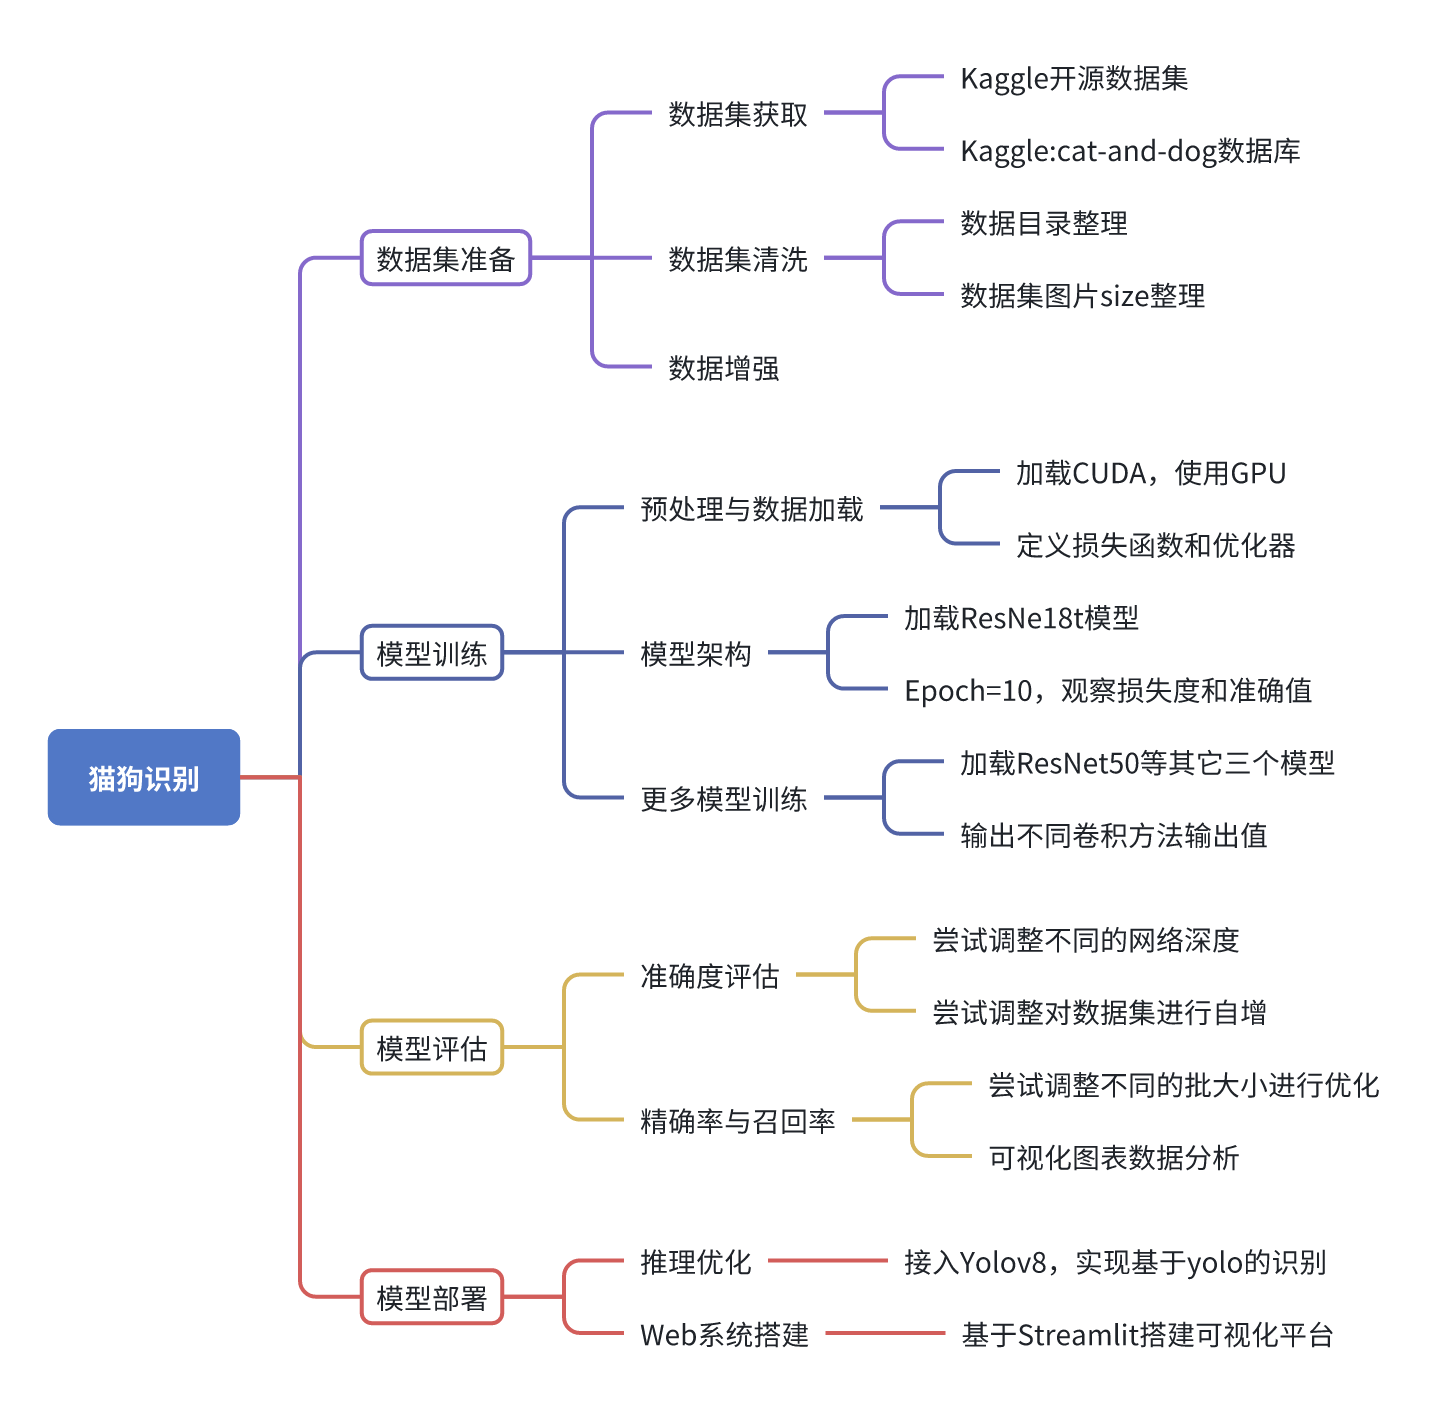
\includegraphics[width=0.6\textwidth]{1746796567985.jpg} %插入图片,[]中设置图片大小,{}中是图片文件名
\caption{项目设计流程图} %最终文档中希望显示的图片标题
\label{图.main2} %用于文内引用的标签
\end{figure}

\begin{CJK*}{GBK}{hei}
\zihao{5}
\vskip 1mm
\section{任务介绍}
\textbf{猫狗识别项目的基本介绍}:
\end{CJK*}

本项目旨在构建一个基于深度学习的猫狗图像识别系统,能够准确判断输入图像中的动物是猫还是狗。该任务本质上是一个二分类问题,在图像分类和动物识别等实际应用场景中具有广泛的应用价值,如宠物管理、图像检索、智能安防等。为实现较高的分类准确率和良好的模型泛化能力,项目在模型结构、训练策略和数据处理等多个方面进行了深入探索和优化。

具体而言,项目以 Pytorch + NetRes 为基础框架,重点围绕以下四个方向展开:

\begin{itemize}
  \item \textbf{网络深度的调整:} 本项目尝试使用不同深度的模型结构(如 YOLOv8n、YOLOv8s、YOLOv8m 等),评估网络层数对特征提取能力与模型性能的影响。通过实验对比,选择最适合猫狗识别任务的深度配置,以在性能与效率之间取得良好平衡。
  
  \item \textbf{批大小的优化:} 批大小对模型的训练过程、收敛速度和最终效果有显著影响。项目中系统地测试了不同的批大小设置,并结合训练曲线和验证集表现进行对比分析,寻找最优的训练参数组合,以提升模型稳定性和训练效率。
  
  \item \textbf{数据集自增处理:} 为了提升模型对不同姿态、光照、背景干扰等复杂场景的适应能力,项目对原始数据集进行了多种形式的数据增强操作,如图像旋转、平移、裁剪、颜色扰动等,从而有效增加样本多样性,缓解模型过拟合问题,提高模型在未知数据上的鲁棒性。
  
  \item \textbf{卷积方法对比实验:} 项目还针对不同的卷积操作进行了实验,包括标准卷积与深度可分离卷积等,分析其对模型参数量、推理速度及分类准确率的影响,进一步优化模型结构,提高整体性能。
\end{itemize}

综上所述,本项目除了完成了猫狗识别系统的构建与部署这一基本任务,还围绕核心参数(批大小、网络深度)和关键模块(网络模型)进行了系统性的实验和优化。相关工作为后续更复杂的图像识别任务(如多类宠物识别、姿态分析等)打下了坚实基础,也为深度学习在小样本二分类场景下的实践提供了可借鉴的经验。



{\begin{CJK*}{GBK}{hei}\subsection{模型构建与关键数学原理}\end{CJK*}}

本项目基于深度卷积神经网络(CNN)实现对猫狗图像的二分类识别。在实验中,我们尝试了不同的网络深度(例如不同层数的 ResNet 架构),以分析深层模型对识别性能的影响;同时尝试了不同的批大小(batch size)对训练稳定性和收敛速度的优化效果。此外,我们还采用数据增强手段提升模型的泛化能力,并分析了不同卷积结构对特征提取结果的影响。本节将从数学角度介绍本项目所涉及的核心深度学习原理和公式。

\subsubsection{卷积操作(Convolution Operation)}

卷积层是卷积神经网络的基础组件,其作用是提取输入图像中的局部特征。二维卷积操作可表示为:

\begin{equation}
Y(i, j) = \sum_{m=0}^{M-1} \sum_{n=0}^{N-1} X(i+m, j+n) \cdot K(m, n)
\end{equation}

其中,$X$ 为输入特征图,$K$ 为卷积核,$Y$ 为输出特征图,$(i,j)$ 为特征图中某一位置。

\subsubsection{残差连接结构(Residual Connection)}

为了解决深层网络训练中的退化问题,我们采用了 ResNet 架构,其核心思想是引入恒等映射(Identity Mapping):

\begin{equation}
y = \mathcal{F}(x, \{W_i\}) + x
\end{equation}

其中,$x$ 表示输入特征,$\mathcal{F}$ 表示残差映射,$W_i$ 表示网络中的卷积权重参数。该结构有助于信息在深层网络中直接传递,提高训练效率。

\subsubsection{激活函数(Activation Function)}

为引入非线性能力,我们在每个卷积层后使用 ReLU 激活函数,其定义为:

\begin{equation}
f(x) = \max(0, x)
\end{equation}

ReLU 能有效缓解梯度消失问题,加快模型收敛速度。

\subsubsection{损失函数(Loss Function)}

本项目为二分类任务,采用交叉熵损失函数作为优化目标:

\begin{equation}
\mathcal{L}_{CE} = - \left[ y \cdot \log(\hat{y}) + (1 - y) \cdot \log(1 - \hat{y}) \right]
\end{equation}

其中 $y \in \{0, 1\}$ 为真实标签,$\hat{y}$ 为模型预测概率。该损失函数在二分类任务中具有良好的判别能力。

\subsubsection{批归一化(Batch Normalization)}

为加速训练并提升稳定性,我们在卷积层后加入了批归一化操作,其公式如下:

\begin{equation}
\hat{x}_i = \frac{x_i - \mu_B}{\sqrt{\sigma_B^2 + \epsilon}}, \quad y_i = \gamma \hat{x}_i + \beta
\end{equation}

其中 $\mu_B$ 与 $\sigma_B^2$ 分别为小批量均值与方差,$\gamma$ 和 $\beta$ 为可学习参数。

\subsubsection{小批量随机梯度下降(Mini-batch SGD)}

模型训练使用 mini-batch SGD 优化器进行参数更新,更新公式如下:

\begin{equation}
\theta_{t+1} = \theta_t - \eta \cdot \frac{1}{B} \sum_{i=1}^{B} \nabla_\theta \mathcal{L}(x_i, y_i; \theta)
\end{equation}

其中 $\theta$ 表示当前模型参数,$\eta$ 为学习率,$B$ 为批大小,$\mathcal{L}$ 为损失函数。我们通过调整不同的批大小进行实验对比,以验证其对模型收敛和准确率的影响。


本节从数学公式角度总结了猫狗识别项目中使用的主要模型结构与训练机制。这些理论基础支撑了我们对网络深度、批大小、卷积变种结构等关键参数的调优实验,也为后续分析提供了理论依据。

\begin{table}[htbp]
\centering
{\begin{CJK*}{GBK}{hei}表1\quad 本项目所使用的四种模型及对比实验维度\end{CJK*}}
\vspace{-2.5mm}
\begin{scriptsize} % 或 \small
\begin{tabular}{lcccc}
\toprule
模型名称 & 网络深度 & 批大小优化 & 数据集自增 & 卷积结构对比 \\
\midrule
ResNet18 & 较浅(18层) & √ & √ & 部分比较 \\
ResNet34 & 中等(34层) & √ & √ & 有 \\
ResNet50 & 深层(50层) & √ & √ & 全面对比 \\
自定义卷积结构 & 自设结构 & √ & √ & 聚焦卷积核变体 \\
\bottomrule
\end{tabular}
\end{scriptsize}
\label{tab1}
\end{table}

\section{关键实现技术}
{\begin{CJK*}{GBK}{hei}本节将详细介绍本项目在模型开发与部署过程中所使用的关键技术实现,包括数据预处理、模型训练流程、可视化界面构建及部署策略等。\end{CJK*}}

\subsection{数据预处理与增强}
为了提升模型的泛化能力,我使用了多种数据增强方法,包括随机裁剪、旋转、水平翻转以及颜色抖动。基于 PyTorch 的 \texttt{torchvision.transforms} 模块构建了数据管道,在训练集上动态增强图像。

\subsection{模型训练与评估}
本项目使用 PyTorch 框架构建并训练 ResNet 系列模型。训练流程包括模型定义、损失函数配置、优化器选择(Adam)、训练轮数控制、模型保存与加载机制。通过监控训练损失与验证准确率,实现模型性能的持续评估与调优。

\subsection{可视化界面与部署}
基于 Streamlit 框架构建了一个交互式 Web 界面,用户可上传图片进行猫狗识别并实时查看预测结果。界面同时集成了模型预测可视化(如类别概率柱状图)与图片预览功能,提升了系统的易用性与直观性。

\begin{figure}[htbp]
\centering
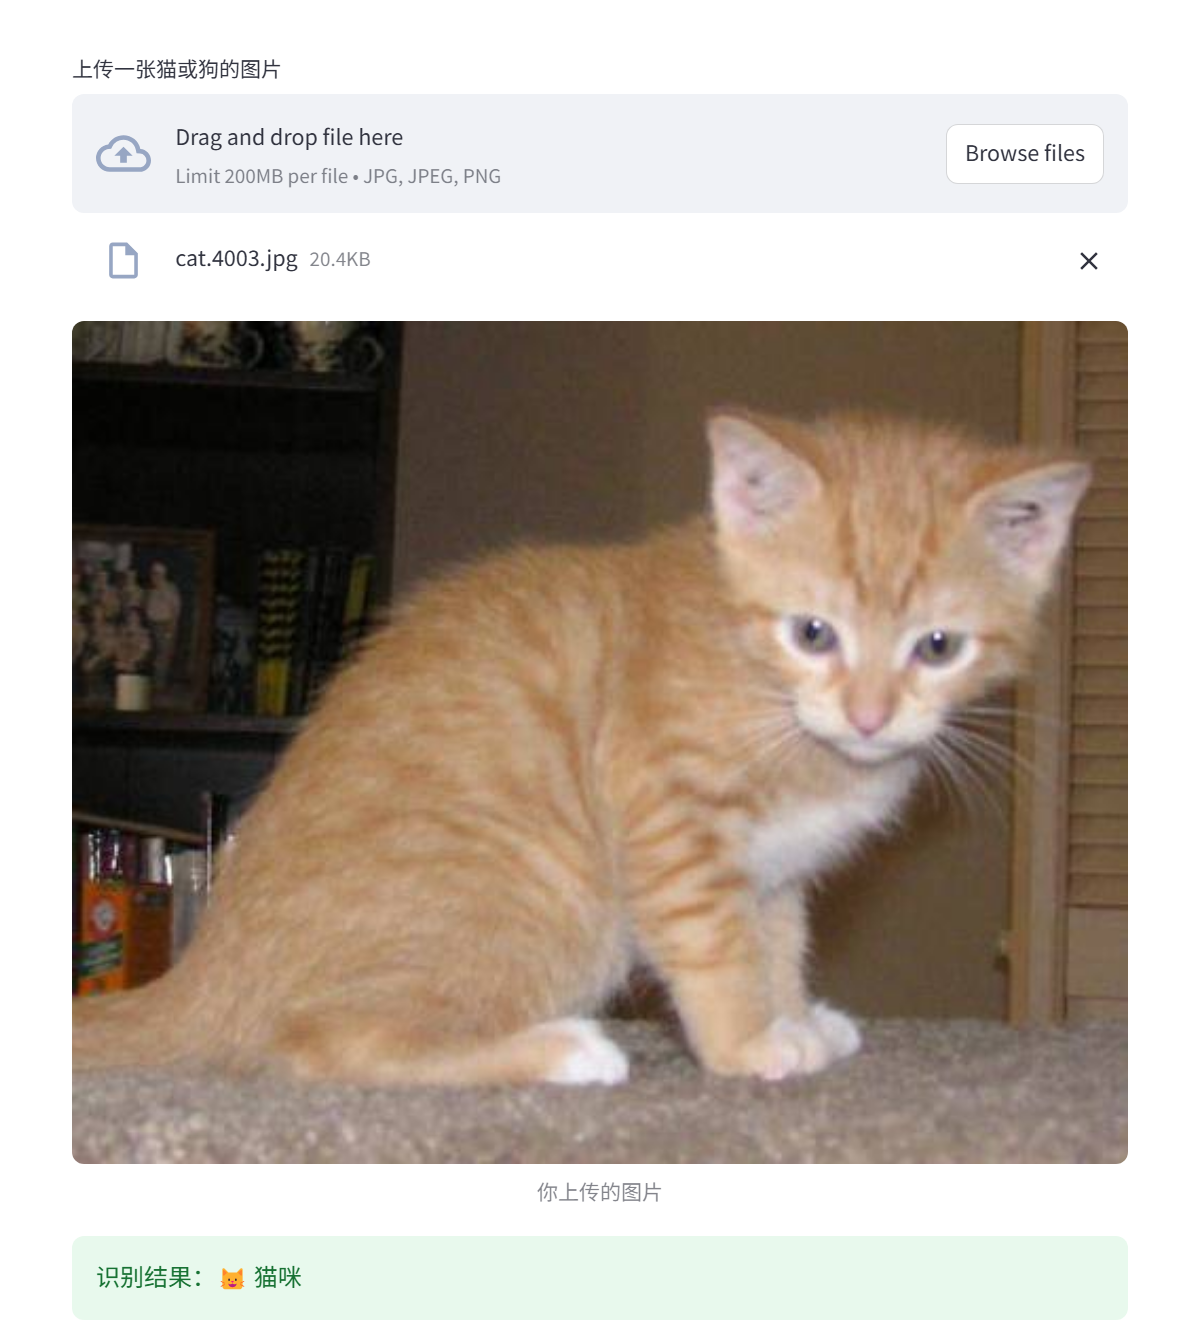
\includegraphics[width=0.9\linewidth]{web_demo.jpg}
{\begin{CJK*}{GBK}{hei} \caption{图2\quad 猫狗识别AI的Web可视化界面展示} \end{CJK*}}
\label{Fig:web_demo}
\end{figure}

\subsection{训练日志与模型管理}
训练过程中的日志信息(如损失变化、准确率曲线)使用 Matplotlib 绘图保存,同时通过 PyTorch 的模型保存机制 \texttt{torch.save()} 将权重文件固化,便于后续加载与部署。以下是预测分析代码predict.py核心部分

\begin{lstlisting}[language=Python, caption={代码1\quad 图像分类预测函数}, label={code:predict}, frame=single, breaklines=true]
def predict_image(image_path):
    transform = transforms.Compose([
        transforms.Resize(224),
        transforms.ToTensor(),
        transforms.Normalize(mean=[0.485, 0.456, 0.406], std=[0.229, 0.224, 0.225])
    ])

    # 加载模型
    device = torch.device("cuda" if torch.cuda.is_available() else "cpu")
    model = create_model()
    model.load_state_dict(torch.load('cat_dog_classifier.pth'))
    model.to(device)

    img = Image.open(image_path)
    img = transform(img).unsqueeze(0).to(device)

    model.eval()
    with torch.no_grad():
        outputs = model(img)
        _, predicted = torch.max(outputs, 1)

    class_names = ['cats', 'dogs']
    predicted_class = class_names[predicted.item()]
    print(f"预测分类: {predicted_class}")
\end{lstlisting}

{\begin{CJK*}{GBK}{hei}\section{模型验证与复现}\end{CJK*}}

为了验证本项目中猫狗识别系统的有效性,并帮助读者更好地理解和复现模型,我在本节中提供了完整的复现实验流程,包括运行环境、依赖配置、代码结构与使用方法。此外,项目已在 GitHub 上开源,地址如下:

\begin{center}
\url{https://github.com/yinlin712/dog-cat-classifiy/}
\end{center}

GitHub的master分支仅仅是完成最基础的猫狗识别任务,另外在项目的v2分支中实现了不同模型,批大小不同等高级目标实现。

\subsection*{1. 运行环境配置}

建议在以下环境中运行项目代码:

\begin{itemize}
  \item 操作系统:Windows 10 / Ubuntu 20.04
  \item Python版本:3.8及以上,推荐采用Anaconda
  \item PyTorch版本:1.12+(需支持GPU,如不支持CUDA请换成CPU)
  \item 依赖库:torchvision、Pillow、matplotlib、streamlit、numpy 等
\end{itemize}

所有依赖可通过如下命令一次性安装:

\begin{lstlisting}[language=bash]
pip install -r requirements.txt
\end{lstlisting}

\subsection*{2. 数据集准备}

本项目使用的猫狗图像数据集可参考 Kaggle 提供的猫狗分类数据集。数据应按照如下结构放置于 `dataset/` 目录下:

\begin{lstlisting}[language=bash]
dataset/
├── train/
│   ├── cats/
│   └── dogs/
├── val/
│   ├── cats/
│   └── dogs/
\end{lstlisting}

\subsection*{3. 模型训练与测试}

运行以下命令可开始训练模型(以 ResNet18 为例):

\begin{lstlisting}[language=bash]
python train.py --model resnet18 --epochs 20 --batch-size 32
\end{lstlisting}

训练完成后模型将保存在 `cat_dog_classifier.pth` 文件中。使用如下命令进行测试预测:

\begin{lstlisting}[language=bash]
python predict.py --image test.jpg
\end{lstlisting}

\subsection*{4. Web 可视化平台}

本项目提供了一个基于 Streamlit 的可视化平台,可供用户直接上传图片进行分类预测。运行如下命令启动网页界面:

\begin{lstlisting}[language=bash]
streamlit run app.py
\end{lstlisting}

启动后将在本地打开 Web 页面,如图\ref{fig:web_demo} 所示,用户可以上传任意图片进行测试分类。


\vspace{3mm}
{\begin{CJK*}{GBK}{hei}该章节旨在实现完整复现流程的公开透明,提升模型的实用性与可拓展性。\end{CJK*}}


\section{总结与展望}

本项目基于深度学习技术,采用了卷积神经网络(CNN)来实现猫狗图像的二分类任务。通过采用经典的ResNet系列模型(ResNet18、ResNet34、ResNet50),并结合数据增强技术和优化的训练流程,成功实现了高精度的猫狗分类系统。我们详细介绍了从数据预处理到模型训练的每个关键步骤,并展示了如何利用PyTorch框架进行实现。

在项目中,我使用了交叉熵损失函数和Adam优化器来加速模型的训练过程,并通过批大小优化和网络深度调整等技术手段提升了模型的性能。对于不同的网络深度(如ResNet18、ResNet34、ResNet50)以及卷积结构的变化,进行了实验对比,并得到了较为稳定且优秀的结果。此外,还探索性地对YOLOv8进行集成,探索了目标检测任务的潜力。

在此基础上,本文为读者提供了代码实现、模型训练流程和可视化的Streamlit Web界面,确保读者能够复现并根据实际需要进行修改和优化。项目的开源地址为:\url{https://github.com/yinlin712/dog-cat-classifiy/},提供了完整的实现代码及模型训练过程,供感兴趣的研究者进一步探索。

尽管本项目在猫狗分类任务中取得了不错的效果,但仍有一些方面可以进一步优化。未来的工作可以从深度学习模型的优化入手,尝试更多的网络结构,如DenseNet或VGG,以进一步提高分类精度。此外,进一步扩大数据集规模,使用更多的图片来源,并进行更丰富的数据增强,如旋转、裁剪等,也可以提升模型的泛化能力。同时,尝试不同模型的集成方法,如Bagging和Boosting,结合多个模型的优势,进一步提升分类性能。迁移学习也是未来的一个研究方向,特别是将训练好的模型应用于类似任务,如动物识别、植物识别等,探索迁移学习的效果。

通过这些进一步的工作,我期望能够推动猫狗图像识别系统在实际应用中的发展,并为更多的计算机视觉任务提供参考和启发。


% \textbf{正文文字要求语句通顺,无语法错误,结构合理,条理清楚,不影响审稿人、读者阅读理解全文内容。以下几类问题请作者们特别注意}:

% 1) 文章题目应明确反映文章的思想和方法;文字流畅,表述清楚;

% 2) 中文文字、英文表达无语法错误;

% 3) 公式中无符号、表达式的疏漏,没有同一个符号表示两种意思的情况;

% 4) 数学中使用的符号、函数名用斜体;

% 5) 使用的量符合法定计量单位标准;

% 6) 矢量为黑体,标量为白体;

% 7) 变量或表示变化的量用斜体;

% 8) 图表规范,量、线、序无误,位置正确(图表必须在正文中有所表述后出现,即{\ldots}如图1所示)(注意纵、横坐标应有坐标名称和刻度值)。

% 9) 列出的参考文献必须在文中按顺序引用,即参考文献顺序与引用顺序一致,各项信息齐全(格式见参考文献部分);

% 10) 首次出现的缩写需写明全称,首次出现的符号需作出解释。

% 11) 图的图例说明、坐标说明全部用中文或量符号。

% \textbf{12) 图应为矢量图。}

% 13) 表中表头文字采用中文。

% 14) 公式尺寸:

% 标准:10.5磅

% 下标/上标:5.8磅

% 次下标/上标:4.5磅

% 符号:16磅

% 次符号:10.5磅

% 15) 组合单位采用标准格式,如:``pJ/bit/m$^{4}$''应为 ``pJ/(bit$\cdot
% $m$^{4})$''

% {\begin{CJK*}{GBK}{hei}\textbf{定理1}.\end{CJK*}}\quad ******. *定理内容.*

% [``定义''、``假设''、``公理''、``引理''等的排版格式与此相同,详细定理证明、公式可放在附录中]

% {\begin{CJK*}{GBK}{fs}证明\end{CJK*}}.\quad  *证明过程.* [``例 x''等的排版格式相同]

% \rightline {证毕.}

% \begin{figure}[htbp]
% \centerline{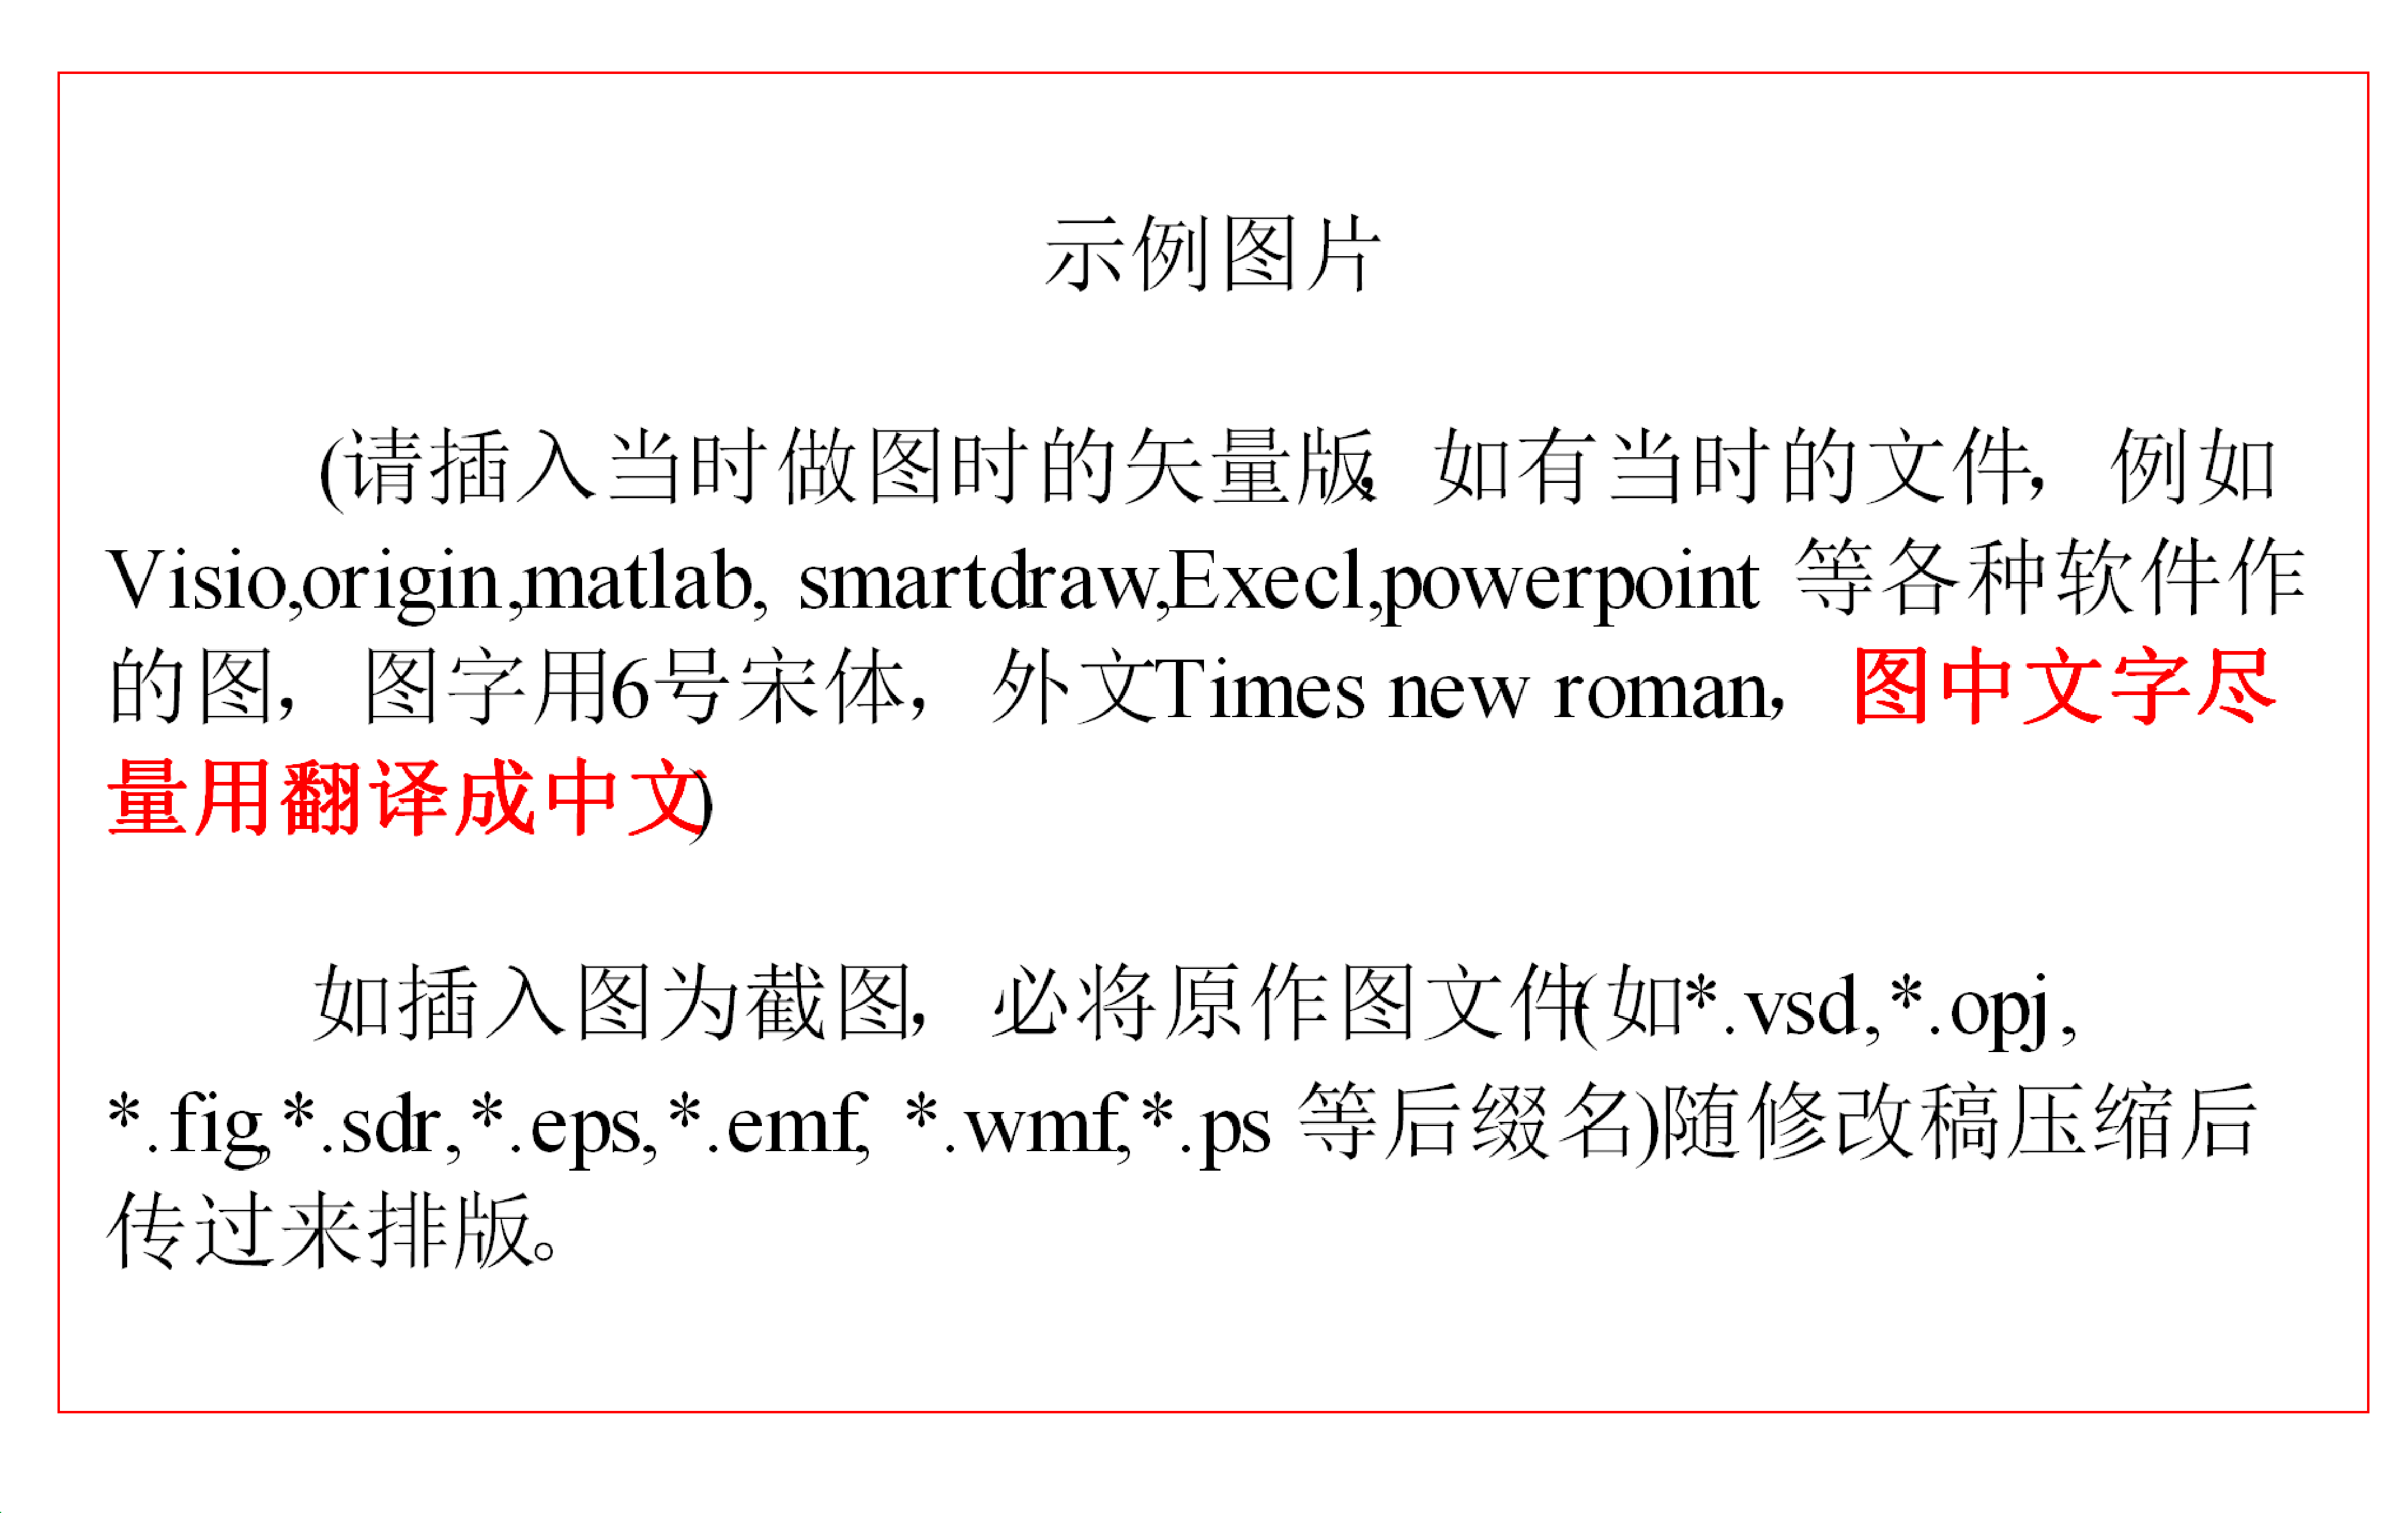
\includegraphics[width=3.15in,height=1.98in]{CJC1.pdf}}
% 图X\quad  图片说明 *字体为小5号,图片应为黑白图,图中的子图要有子图说明*
% \label{fig1}
% \end{figure}

% \begin{table}[htbp]
% \centering {\begin{CJK*}{GBK}{hei}表X\quad 表说明 *表说明采用黑体*\end{CJK*}}
% \vspace {-2.5mm}
% \begin{center}
% \begin{tabular}{ll}
% \toprule
% *示例表格*&*第1行为表头,表头要有内容* \\
% \hline
% &
%  \\
% &
%  \\
% &
%  \\
% &
%  \\
% \bottomrule
% \end{tabular}
% \label{tab1}
% \end{center}
% \end{table}

% \begin{CJK*}{GBK}{hei}过程X.\end{CJK*}\quad 过程名称

% {\zihao{5-}*《计算机学报》的方法过程描述字体为小5号宋体,IF、THEN等伪代码关键词全部用大写字母,变量和函数名称用斜体*}


% \begin{CJK*}{GBK}{hei}算法\textbf{Y}\end{CJK*}.\quad 算法名称.
% \zihao{5-}{

% \noindent 输入:{\ldots} {\ldots}

% \noindent 输出:{\ldots} {\ldots}

% *《计算机学报》的算法描述字体为小5号宋体, IF、THEN等伪代码关键词全部用大写字母,变量和函数名称用斜体*}

\vspace {3mm}
\zihao{5}{
\noindent \begin{CJK*}{GBK}{hei}致\quad 谢\end{CJK*}\quad \begin{CJK*}{GBK}{kai} 感谢Kaggle对本项目设计提供的数据支持 \end{CJK*}}


\vspace {5mm}
\centerline
{\zihao{5}
\begin{CJK*}{GBK}{hei}参~考~文~献\end{CJK*}}

\begin{thebibliography}{99}
\zihao{5-} \addtolength{\itemsep}{-1em}
\vspace {1.5mm}

\bibitem[1]{1} 
Szegedy, C., Vanhoucke, V., Ioffe, S., Shlens, J., & Wojna, Z. (2016). Rethinking the inception architecture for computer vision. \textit{Proceedings of the IEEE Conference on Computer Vision and Pattern Recognition (CVPR)}, 2818-2826. 

\bibitem[2]{2} 
周永彬, 冯登国. RFID安全协议的设计与分析. \textit{计算机学报}, 2006, 29(4): 581-589. \newline
Zhou Yong-Bin, Feng Deng-Guo. Design and analysis of cryptographic protocols for RFID. \textit{Chinese Journal of Computers}, 2006, 29(4): 581-589.

\bibitem[3]{3} 
He, K., Zhang, X., Ren, S., & Sun, J. (2016). Deep residual learning for image recognition. \textit{Proceedings of the IEEE Conference on Computer Vision and Pattern Recognition (CVPR)}, 770-778.

\bibitem[4]{4} 
P. P. Vaidyanathan, & A. S. Wagstaff. Image Processing Using Wavelet Transforms. \textit{IEEE Transactions on Signal Processing}, 2004, 52(7): 2139-2151.

\bibitem[5]{5} 
李明. 深度学习应用于猫狗图像分类的研究与实践. \textit{计算机科学与探索}, 2020, 14(3): 102-108. \newline
Li Ming. Research and practice of deep learning in cat-dog image classification. \textit{Computer Science and Exploration}, 2020, 14(3): 102-108.

\bibitem[6]{6} 
Simonyan, K., & Zisserman, A. (2014). Very deep convolutional networks for large-scale image recognition. \textit{Proceedings of the International Conference on Learning Representations (ICLR)}, 1-14.

\bibitem[7]{7} 
王强, 刘涛. 基于卷积神经网络的图像分类研究综述. \textit{图像与视觉计算}, 2019, 21(5): 45-60. \newline
Wang Qiang, Liu Tao. A survey on image classification based on convolutional neural networks. \textit{Image and Vision Computing}, 2019, 21(5): 45-60.

\end{thebibliography}

% \noindent {\zihao{5}\bf{附录X}.}

% {\zihao{5-}\setlength\parindent{2em}
% \textbf{附录内容}置于此处,字体为小5号宋体。附录内容包括:\textbf{详细的定理证明、公式推导、原始数据}等。\\

% 如需访问数据集,请点击以下链接:[Kaggle Cat and Dog Dataset](https://www.kaggle.com/datasets/tongpython/cat-and-dog)
% }

\begin{strip}
\end{strip}

\begin{biography}[lby.jpg]
\noindent
\textbf{Li Bo-You},Junior.沈阳理工大学计算机科学与技术专业大三在读学生,正在学习机器学习、深度学习、Python开发等领域的内容。A Shenyang Ligong University Junior,majoring in Computer Science and Technology. He focus is on Machine Learning、Deep Learning、Python Development.

\end{biography}

% \begin{biography}[yourphotofilename.jpg]
% \noindent
% \textbf{Second B. Author} *英文作者介绍内容包括:出生年,学位(或目前学历),职称,主要研究领域(\textbf{与中文作者介绍中的研究方向一致})。*
% *字体为小5号Times New Roman*
% \end{biography}
% \begin{strip}
% \end{strip}
% \zihao{5}
% \noindent \textbf{Background}

% \zihao{5-}{
% \setlength\parindent{2em}
% *论文背景介绍为\textbf{英文},字体为小5号Times New Roman体*

% 论文后面为400单词左右的英文背景介绍。介绍的内容包括:

% 本文研究的问题属于哪一个领域的什么问题。该类问题目前国际上解决到什么程度。

% 本文将问题解决到什么程度。

% 课题所属的项目。

% 项目的意义。

% 本研究群体以往在这个方向上的研究成果。

% 本文的成果是解决大课题中的哪一部分,如果涉及863$\backslash
% $973以及其项目、基金、研究计划,注意这些项目的英文名称应书写正确。}

\end{CJK*}
\end{document}


